%%%%%%%%%%%%%%%%%%%%%%%%%%%%%%%%%%%%%%%%%%%%%%%%%%%%%%%%%%%%%%%%%%%%%%%
%%%%%%%%%%%%%%%%%%%%%%%%%%%%%%%%%%%%%%%%%%%%%%%%%%%%%%%%%%%%%%%%%%%%%%%
\deelmetoef{Module 1}{Inleiding}{Module 1. Inleiding}{Oplossingen module 1}{Oplossingen module 1}
\label{sec:inl}
%%%%%%%%%%%%%%%%%%%%%%%%%%%%%%%%%%%%%%%%%%%%%%%%%%%%%%%%%%%%%%%%%%%%%%%
%%%%%%%%%%%%%%%%%%%%%%%%%%%%%%%%%%%%%%%%%%%%%%%%%%%%%%%%%%%%%%%%%%%%%%%

\begin{samenvatting}
Tijdens dit project maken we een smartphone app waarmee je je hartslag kan meten. We leggen later uit waarom het belangrijk is af en toe je hartslag te meten en waarom we ervoor kiezen dit met een app te doen. Daarna bekijken we wat een hartslag precies is en hoe we die met onze smartphone kunnen meten.
\end{samenvatting}
%

%%%%%%%%%%%%%%%%%%%%%%%%%%%%%%%%%%%%%%%%%%%%%%%%%%%%%%%%%%%%%%%%%%%%%%%
\section{Wat en waarom?}
\label{sec:Mod1_Sec1}
%%%%%%%%%%%%%%%%%%%%%%%%%%%%%%%%%%%%%%%%%%%%%%%%%%%%%%%%%%%%%%%%%%%%%%%
%
De hartslag duidt aan hoe vaak je hart klopt per minuut. Tijdens het sporten is het belangrijk je hartslag in het oog te houden. Een te hoge hartslag wijst op een te hoge inspanning, en kan mogelijks gevaarlijk zijn. Bovendien kan een (te) hoge hartslag in rust wijzen op aandoeningen zoals een overactieve schildklier, bloedarmoede of bloedverlies, een longaandoening enz. Regelmatig je hartslag controleren is dus de boodschap.

Om je hartslag te meten gebruiken we meestal een bloeddrukmeter.

\begin{minipage}{.5\linewidth}
	\gewonefiguur{width=\linewidth}{module1/patient}
\end{minipage} 
\begin{minipage}{.5\linewidth}
	\gewonefiguur{width=\linewidth}{module1/hartslagmonitor}
\end{minipage} 

Zo'n bloeddrukmeter is een gespecialiseerd toestel dat meestal enkel een dokter of iemand met hartklachten ter beschikking heeft. Bovendien is het nogal omslachtig een bloeddrukmeter tijdens het sporten mee te nemen, gezien dit niet echt een draagbaar toestel is.

\gewonefiguur{width=.5\linewidth}{module1/lopermethartslagmeter}

Een alternatief voor de bloeddrukmeter is de hartslagmeter. 

\begin{minipage}{.5\linewidth}
	\gewonefiguur{width=\linewidth}{hartslagmeter}
\end{minipage} 
\begin{minipage}{.5\linewidth}
	\gewonefiguur{width=\linewidth}{module1/loper-met-dure-loopband}
\end{minipage} 

Een hartslagmeter kan je wel makkelijk meenemen bij het sporten. Bovendien geeft de hartslagmeter ook \textquotedblleft real time feedback\textquotedblright; dat wil zeggen dat je op elk moment quasi onmiddellijk je hartslag kan zien. Maar wellicht ligt de aanschaf van een hartslagmeter niet binnen het budget van elke leerling of student?

Daarom bouwen wij in dit project onze eigen smartphone app, waarmee we snel, eenvoudig en redelijk accuraat onze hartslag kunnen meten, zonder nood aan gespecialiseerde toestellen.

\gewonefiguur{width=.5\linewidth}{module1/loper}

\section{De hartslag}
\label{sec:Mod1_Sec2}

Je hart is een spier die samentrekt om je bloed in je lichaam rond te pompen. De hartslag is de pompbeweging van je hart. In de volksmond is de hartslag ook het aantal samentrekkingen van je hart per minuut, of anders gezegd het aantal keer dat je hart klopt per minuut.

De hartslag in rust van een volwassene varieert tussen 60 en 100 slagen per minuut. De Maximale Hartslag (aangeduid als $MH$) is de hoogste hartslag die je lichaam aan kan gedurende fysische activiteit. De maximale hartslag varieert naargelang je leeftijd en kan berekend worden met de volgende vuistregel

\begin{equation*}
MH = 220-LT
\end{equation*}

met volgende notatie:
\begin{itemize}
	\item MH: maximale hartslag met als eenheid slagen per minuut of \textquotedblleft beats per minute \textquotedblright (kortweg: bpm). 
	Dit noteren we als MH [bpm].
	\item LT [jaar]: leeftijd
\end{itemize}

Tijdens het sporten houd je best je hartslag tussen 55 en 85\% van je maximale hartslag. 

Voor een volwassene van 20 jaar oud is het aangeraden hartslagbereik tijdens het sporten dus tussen 110 en 170 bpm.
Voor een volwassene van 50 jaar oud is het aangeraden hartslagbereik tijdens het sporten lager, nl. tussen 94 en 145 bpm.

Dit kunnen we in tabelvorm schrijven als volgt:

\begin{center}	
	\begin{tabular}{c|ccc}
		LT & MH & 0,55*MH & 0,85*MH \\
		\hline
		20 & 200 & 110 & 170 \\
		50 & 170 & 94 & 145 
	\end{tabular}
\end{center}

\begin{oef}
Bereken de maximale hartslag $MH$ en het ideale hartslagbereik tijdens het sporten van een volwassene van 
\begin{itemize}
	\item 18 jaar
	\item 30 jaar
	\item 65 jaar
\end{itemize}
\end{oef}
\oplos{\begin{itemize}
		\item $MH_{18}=202$ en hartslagbereik tussen 111,1 en 171,7
		\item $MH_{30}=190$ en hartslagbereik tussen 104,5 en 161,5
		\item $MH_{65}=155$ en hartslagbereik tussen 85,25 en 131,75
	\end{itemize}
}

\begin{oef}Maak ook een grafiek die de maximale hartslag $MH$ uitzet in functie van de leeftijd $LT$. 

Welke grootheid komt op de $x$-as? Wat is de eenheid? 

Welke grootheid komt op de $y$-as? Wat is de eenheid?
\end{oef}
\oplos{
	\begin{tikzpicture}[domain=0:100]
	\begin{axis}[axis lines=middle,xmax=110,ymin=-1,ymax=240,
		x label style={at={(axis description cs:0.5,-0.1)},anchor=north},
		y label style={at={(axis description cs:-0.1,.5)},rotate=90,anchor=south},
		xlabel={LT (Jaar)},ylabel={MH (bpm)}]
	\addplot[domain=0:100] {220-x} node[left]{$MH=220-LT$};
	\end{axis}
	\end{tikzpicture}
}

De hartslag, of het rondpompen van je bloed, kan je voelen wanneer je je hand op je hart legt. Maar ook in je hals of aan je pols kan je je hartslag voelen. Handmatig meten van de hartslag kan je doen door twee gestrekte vingers op de pols (van jezelf of van een ander persoon) of in de hals (tegen de halsslagader) te plaatsen. Hier voel je de hartslag heel goed. Tel je gedurende 15 seconden het aantal hartslagen en vermenigvuldig je dit getal met vier, dan heb je een goede indicator van het aantal keer dat je hart pompt per minuut.

\begin{opdracht}{Opdracht: Je eigen hartslag meten}
	\begin{enumerate}
		\item Handmatig \\
		\begin{itemize}
			\item Meet je eigen hartslag door twee gestrekte vingers in je hals te plaatsen. 
			\item Tel het aantal keer dat je hart pompt gedurende 15 seconden en vermenigvuldig dit getal met vier.
		\end{itemize}
		\item Met de science journal app \footnote{Tip voor leerkachten:
			Het gebruik van de app Science Journal kan je demonstreren door je smartphone scherm te projecteren op je computer. Hiervoor kan je het programma (op je pc) en de app (op je smartphone) Vysor gebruiken wanneer je smartphone met een USB kabel met de pc verbonden is.}\\	
			\begin{minipage}{.6\linewidth}
				Als je moeite hebt om het aantal hartslagen te tellen, kan je ook gebruik maken van de smartphone app \textquoteleft Science journal\textquoteright. De app kan je downloaden in de Google Play Store.
				\begin{itemize}
					\item Start een nieuw experiment en meet het omgevingsgeluid, zoals in de figuur hiernaast. 
					\item Plaats twee gestrekte vingers in je hals en zeg \textquoteleft ja\textquoteright \ elke keer als je een hartslag voelt. 
					\item Doe dit gedurende 15 seconden. 
					\item Tel nadien het aantal pieken dat geregistreerd werd en vermenigvuldig dit aantal met vier om de hartslag te bekomen.
				\end{itemize}
			\end{minipage}	
			\begin{minipage}{.4\linewidth}
				\figuurmetlabel[\label{fig:app_scienceJournal}]{height=8cm}{module1/illustratieScienceJournal}{De app Science journal. Gebruik de luidspreker om je stem en het omgevingsgeluid op te nemen.}
			\end{minipage}	
		
			\begin{minipage}{.6\linewidth}
			\begin{itemize}
				\item De afbeelding hiernaast toont alvast een voorbeeld. 
				\item Voor deze meting tellen we 15 pieken op 15 seconden. 
				\item Na vermenigvuldigen met vier vinden we in dit geval een hartslag van 60 bpm.
			\end{itemize}
			\end{minipage}	
			\begin{minipage}{.4\linewidth}
				\figuurmetlabel[\label{fig:meting_scienceJournal}]{height=8cm}{module1/metingScienceJournal}{Voorbeeld van een geluidsmeting in Science Journal. \newline}
			\end{minipage}	
	\end{enumerate}

	
%	\begin{minipage}{.5\linewidth}
%		
%	\end{minipage}
%	\begin{minipage}{.5\linewidth}
%		\figuurmetlabel[\label{fig:meting_scienceJournal}]{height=12cm}{module1/metingScienceJournal}{Voorbeeld van een geluidsmeting in Science Journal. \newline}
%	\end{minipage}

%	Zo tellen we voor bovenstaande meting 15 pieken op 15 seconden. De hartslag bekomen we door dit aantal te vermenigvuldigen met vier: de hartslag is 60 bpm.

\end{opdracht}

\begin{oef}
	Stel dat je gedurende 10 tellen in plaats van 15 seconden het aantal hartslagen bijhoudt.
	\begin{itemize}
		\item Met welke factor moet je dit aantal vermenigvuldigen om een correcte hartslag in bpm te bekomen? 
	
		\item Wat is de factor bij een telperiode van 20 seconden?
	
		\item Welk voordeel biedt een langere telperiode?
	\end{itemize}
\end{oef}
\oplos{\begin{itemize}
		\item $10~s$: factor $6$
		\item $20~s$: factor $3$
		\item Hoe korter de telperiode, hoe nauwkeuriger je moet tellen. Eventuele telfouten worden immers vermenigvuldigd met de factor. De factor is groter, naarmate de telperiode korter is. Telfouten worden dus groter als de telperiode korter is.
	\end{itemize}
}

Voor heel hoge hartslagen ($>160~bpm$) wordt het quasi onmogelijk de hartslag nog zelf te tellen. Dan moet je een meettoestel gebruiken. In wat volgt maken wij ons eigen meettoestel: een smartphone app waarmee je goedkoop, snel en gemakkelijk je hartslag kan meten.

\section{Overzicht van het project}
\label{sec:Mod1_Sec3}

\subsection{Hoe pakken we dat aan?}
We hebben al gezien dat je het pompen van je hart goed kan voelen aan je pols of in de hals. Een andere \textquotedblleft handige \textquotedblright \ plek voor het waarnemen van je hartslag is je vingertop; ook daar doen zich kleine pulsaties in je aders voor door het pompen van je hart. 

\gewonefiguur{height=10cm}{module1/loperStilstaand}

We gaan hiervoor slim gebruik maken van de camera die in je smartphone ingebouwd is. 
We zullen onze vingertop zachtjes op de lens van de camera plaatsen en daar een video van maken. 
De kleine pulsaties in de aders van je vinger resulteren in kleine veranderingen in de kleur van je vinger. 
Met het blote oog kan je die miniscule kleurveranderingen meestal niet waarnemen, maar de camera van je smartphone kan die subtiele veranderingen wel detecteren. 
De kleurveranderingen in functie van de tijd zijn gerelateerd aan het pompen van je hart. Een grafiek van de kleurverandering in functie van de tijd zie je hieronder. We gebruiken dezelfde strategie als voorheen: we tellen het aantal pieken gedurende 15 seconden en vermenigvuldigen dit getal met vier.

\gewonefiguur{width=\linewidth}{module3/MSExcel_GraphRedValues}

\subsection{De strategie als blokdiagram}

De opeenvolging van uit te voeren stappen kunnen we voorstellen in een blokdiagram, zoals hieronder. Zo zien we grafisch welke stappen we moeten doorlopen om de hartslag te bepalen. Dit geeft een bondig overzicht van het project, zonder dat we nu al precies en in alle detail moeten weten wat in elke stap moet gebeuren. Deze stapsgewijze aanpak vermijdt dat we zouden verdwalen in een overweldigende hoop denkwerk.

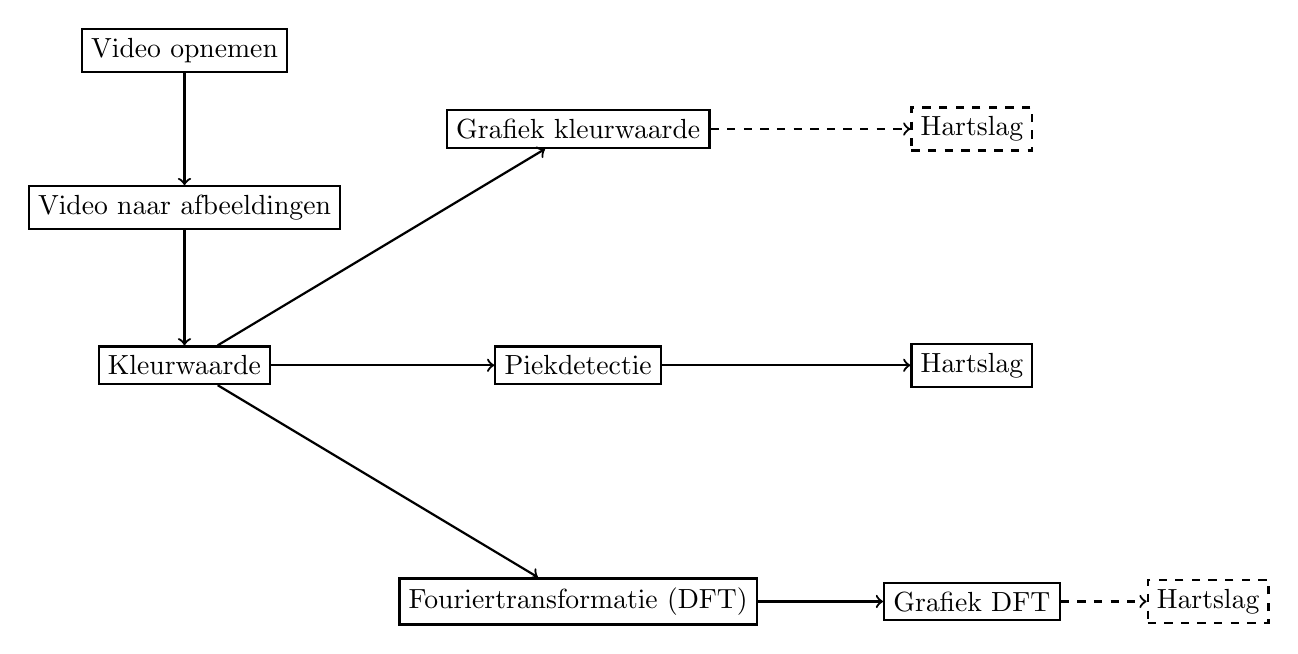
\begin{tikzpicture}[thick]
\node[draw,rectangle] at (0,0) (a) {Video opnemen};
\node[draw,rectangle] at (0,-2) (b) {Video naar afbeeldingen};
\node[draw,rectangle] at (0,-4) (c) {Kleurwaarde};
\node[draw,rectangle] at (5,-1) (d) {Grafiek kleurwaarde};
\node[draw,rectangle,dashed] at (10,-1) (j) {Hartslag};
\node[draw,rectangle] at (5,-4) (e) {Piekdetectie};
\node[draw,rectangle] at (10,-4) (f) {Hartslag};
\node[draw,rectangle] at (5,-7) (g) {Fouriertransformatie (DFT)};
\node[draw,rectangle] at (10,-7) (h) {Grafiek DFT};
\node[draw,rectangle,dashed] at (13,-7) (i) {Hartslag};

\draw[->] (a) -- (b) ;
\draw[->] (b) -- (c) ;

\draw[->] (c) -- (d) ;
\draw[->] (c) -- (e) ;
\draw[->] (c) -- (g) ;

\draw[->,dashed] (d) -- (j) ;
\draw[->] (e) -- (f) ;
\draw[->] (g) -- (h) ;
\draw[->,dashed] (h) -- (i) ;

\end{tikzpicture}

\subsection{De kleurwaarde als functie van de tijd}

We willen de kleurwaarde van je vingertop in functie van de tijd analyseren. 
De camera van je smartphone filmt de kleur van je vingertop.
Een video of een filmpje is in feite niet meer dan een aantal foto's die heel snel na elkaar te voorschijn komen op een scherm.
Die foto's laten ons toe om te bepalen wat de kleurwaarde van je vingertop was op het moment dat de foto werd genomen.
We hebben drie verschillende manieren om vanuit die kleurwaarden de hartslag te bepalen.

\begin{enumerate}
	\item Grafiek \\
	\begin{minipage}{.5\linewidth}
		Een eerste optie is het achter elkaar zetten van de kleurwaarde van alle foto's op die verschillende tijdstippen in een grafiek. Zo zien we het aantal pieken zoals hiernaast. 
	Daaruit kunnen we zelf berekenen wat onze hartslag was op het moment van opname. We doen dit door zoals voorheen het aantal pieken te tellen en te vermenigvuldigen met een factor om het aantal pieken per minuut te bekomen.
	\end{minipage}
	\begin{minipage}{.5\linewidth}
	\gewonefiguur{width=\linewidth}{module3/MSExcel_GraphRedValues}
	\end{minipage}
	\item Automatische piekdetectie \\
	Een tweede manier bestaat uit het automatisch laten herkennen van die pieken door de smartphone. We sparen zo zelf heel wat rekenwerk: de smartphone telt immers het aantal pieken en herleidt dit aantal naar het aantal pieken per minuut.
	Dit bespaart ons heel wat rekenwerk.
	\item Fouriertransformatie \\
	Tenslotte kunnen we beroep doen op de zogenaamde \emph{Fouriertransformatie} die gebaseerd is op wat complexere wiskunde.
	Vooral wanneer de meting een beetje ruizig is, wanneer we de pieken moeilijk kunnen herkennen, zal deze methode nauwkeuriger zijn.
	%TODO vergelijking ruizige en zuivere meting toevoegen
	Hoe deze methode concreet werkt, wordt uitgelegd in Module 4 Sectie \ref{sec:Mod4_Sec3}.
\end{enumerate}

Bij methode 1 en 3 hebben we zelf nog wat denkwerk: we moeten nog gegevens aflezen op een grafiek en daaruit de hartslag bepalen. Daarom staan die twee opties in stippellijn in het blokdiagram. Bij methode 2 doet de smartphone al het lastige reken- en denkwerk; daarom staat die optie in volle lijnen in het blokdiagram.





%\begin{tikzpicture}
%\sbEntree{n1}
%\sbRelier[RecordButton]{n1}
%\sbBlocL{n1}{Video opnemen}{n2}
%%\sbBlocL{n2}{Video naar afbeeldingen}{n3}
%%\sbBlocL{n3}{Kleurwaarde van afbeeldingen}{n4}
%%\sbBlocL{n4}{Grafiek van kleurwaarde ifv tijd}{n5}
%%\sbBlocL{n5}{Piekdetectie kleurwaarden}{}
%%\sbBlocL{n6}{Hartslag berekenen}{n7}
%%\sbSortie[5]{S1}{n7}
%%\sbNomLien[0.8]{S1}{$Hartslag$}
%
%%\sbEntree{E}
%%\sbComp{a}{E}
%%\sbBloc{b}{$H_1$}{a}
%%\sbRelier[$E_1$]{E}{a}
%%\sbBlocL{c}{$H_2$}{b}
%%\sbRelier[$\epsilon$]{a}{b}
%%\sbComph{d}{c}
%%\sbRelier[u]{c}{d}
%%\sbBlocL{e}{$H_3$}{d}
%%\sbBlocL{f}{$H_4$}{e}
%%\sbSortie[5]{S1}{f}
%%\sbRelier{f}{S1}
%%\sbNomLien[0.8]{S1}{$S_1$}
%%\sbDecaleNoeudy[-4]{f}{u}
%%\sbDecaleNoeudy{e}{v}
%%\sbBlocr{r1}{$R_1$}{u}
%%\sbBlocr{r2}{$R_2$}{v}
%%\sbBlocrL{r3}{$R_3$}{r2}
%%\sbRelieryx{f-S1}{r1}
%%\sbRelierxy[n1]{r1}{d}
%%\sbRelieryx{e-f}{r2}
%%\sbRelierxy[n2]{r3}{a}
%\end{tikzpicture}




